\section{Softwarearchitektur}

Im ersten Unterkapitel \ref{erkundungDerKarte} wird zunächst einen Einblick in die Erkundung und die Speicherung der Karte gegeben. Hierfür wird auf die Implementierung und die Aktualisierung der Karte eingegangen sowie auf die Veränderung in Gruppen. Ebenfalls werden die Besonderheiten der wiederholenden Karte und das Koordinatensystem erläutert. Im Kapitel \ref{kap:entscheidungAgenten} wird kurz auf die verwendeten Rollen, die Aufgaben der \textit{Agents} sowie auf die Gruppenbildung und die Wegführung eingegangen. Im Kapitel \ref{kap:lokaleSicht} wird der Unterschied zwischen lokaler und globaler Sicht des Agenten aufgezeigt. Als Abschluss in Kapitel \ref{kap:kommunikation} wird die Kommunikation der Agenten kurz erläutert.

\subsection{Erkundung und Speicherung der Karte} \label{erkundungDerKarte}



In jedem Schritt eines Spiels kann über die \Percepts abgerufen werden, welche Objekte für einen \Agent aktuell sichtbar sind. Wie weit ein \Agent sehen kann, hängt von der Rolle ab. Die von einem \Agent wahrgenommenen \Things werden hierbei mit relativer Distanz zur Position des \Agents angegeben. Wenn sich beispielsweise ein \Obstacle zwei Felder rechts neben dem \Agent befindet, wird dieses im \Percept mit den Koordinaten [2, 0] angegeben. Bewegt sich der \Agent um ein Feld nach rechts, wird das \Obstacle dann im Abstand [1, 0] gesehen. 

Informationen vergangener \Percepts sind nicht verfügbar, d.h. ein \Agent besitzt zunächst einmal kein „Gedächtnis“. Um eine zielgerichtete Planung der \Agents umzusetzen, ist es daher erforderlich, die in jedem \Step wahrgenommenen Sichten zu speichern und so Schritt-für-Schritt eine Karte aufzubauen. \\

\begin{figure}[h]
	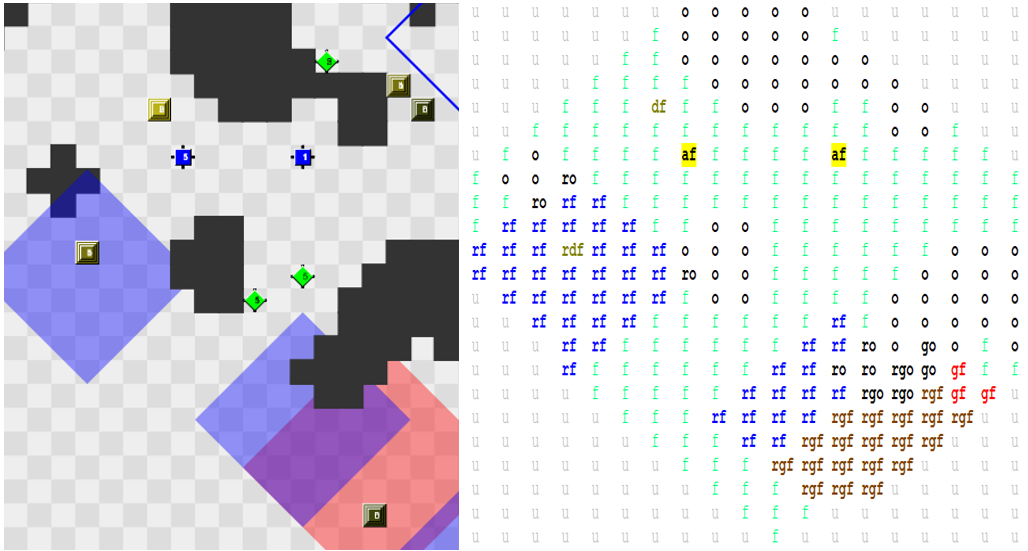
\includegraphics[width=0.8\textwidth]{./Abbildungen/map.png}
	\centering
	\caption{Links: Screenshot der Karte, Rechts: \NextMap-Objekt einer Gruppe mit 2 Agents als Output in eine .txt-Datei. \newline Legende: \underline{a}gent, \underline{d}ispenser, \underline{f}ree, \underline{g}oal zones, \underline{o}bstacles, \underline{r}ole zones, \underline{u}nknown}
\end{figure} 

Es ergeben sich folgende Anforderungen:
\begin{enumerate}
	\item Jeder \Agent soll die in den einzelnen \Steps wahrgenommenen Dinge speichern und auf diese zu einem späteren Zeitpunkt zugreifen können. 
	\item Da manche Informationen der Karte dynamisch sind (z.B. können \Obstacles per \textit{clear()} entfernt werden), ist auch eine Aktualisierung bereits gespeicherter Positionen erforderlich. 
	\item \Agents sollten bestenfalls dieselbe Karte verwenden, sodass jeder \Agent aus der Erkundung / aus dem Wissen der anderen \Agents schöpfen kann.
	\item Die Spiele werden mit einer sich wiederholenden Karte mit unbekannter Kartengröße gespielt. Um eine effiziente Planung zu ermöglichen, soll die Kartengröße ermittelt und die Wiederholungen bei Speicherung der Karte berücksichtigt werden.
\end{enumerate}

\subsubsection{Implementierung} ~\\
Es wurden im Wesentlichen folgende Klassen zur Umsetzung implementiert:
\begin{itemize}
	\item \textit{NextMapTile}: Beschreibung eines einzelnen Feldes mit den Eigenschaften Position, Typ und \Step (Schritt, wann die Position zuletzt gesehen wurde).   
	\item \textit{NextMap}: Beschreibung der Karte als Ganzes durch Speicherung der wahrgenommenen \Things je \Step als \NextMapTiles. \\ Um eine Mehrfach-Belegung einer Position zu ermöglichen (z.B. \GoalZone und \Obstacle auf derselben Position), werden die verschiedenen Typen in jeweils eigenen Datenstrukturen gespeichert (Karte der \Obstacles, Karte der \GoalZones, etc.).
	\item \textit{\NextGroup}: Gruppierung von 1…n \Agents, welche dieselbe Karte nutzen. Jede Gruppe enthält genau ein \NextMap-Objekt. 
\end{itemize}

\subsubsection{Aktualisierung} ~\\
Je \Agent wird geprüft, ob im letzten \Step ein erfolgreicher \move-Befehl ausgeführt wurde. Falls ja, wird die Position des \textit{Agents} aktualisiert und es werden die im \Percept übermittelten \Things zur Karte hinzugefügt bzw. bereits vorhandene Daten aktualisiert. Hierbei werden \Dispenser, \GoalZones, \RoleZones und \Obstacles gespeichert. Andere \Agents und Blöcke werden in der Karte nicht gespeichert, da sich diese meist sehr dynamisch ändern und daher in der langfristigen Wegeplanung nicht relevant sind.

\subsubsection{Gruppen} ~\\
Bei Start des Spiels wird für jeden \Agent eine eigene Gruppe erzeugt, welche genau eine Karte enthält. Alle wahrgenommenen Dinge werden in dieser Karte gespeichert und sind zunächst nur für diesen \Agent sichtbar. 
Wenn sich zwei \Agents während des Spiels in entgegengesetzter Richtung wahrnehmen und sie das einzige Paar sind, welches sich in dieser Richtung und Entfernung sieht (Eindeutigkeit), wird die Gruppe des einen \Agent mit der Gruppe des anderen \Agent zusammengeführt. Hierbei werden alle \Agents sowie alle Daten der Karte übertragen. Sofern in beiden Karten Informationen für dieselben Positionen vorhanden sind, bleibt nur das aktuellere \NextMapTile erhalten und das ältere wird verworfen. Aktualisierungen der Karte aller \Agents sind anschließend für alle anderen \Agents der Gruppe sichtbar.

Bei den im Fachpraktikum gespielten Turnieren erfolgte die erste Zusammenführung von Gruppen meist nach nur wenigen Schritten. Innerhalb des ersten Drittel des Spiels haben die Agents i.d.R. in nur noch einer Gruppe agiert, sodass die gemeinsame Datenbasis der Karte über einen Großteil des Spiels genutzt werden konnte. 

\subsubsection{Wiederholende Karte} ~\\
Typischerweise werden die Spiele des \textit{Multi Agent Programming Contest 2022} mit einer randlosen Karte gespielt. Die Größe der Karte ist zu Beginn nicht bekannt und die Grenzen sind für die \Agents bei der Erkundung der Karte nicht erkennbar, sodass sie sich auf einer scheinbar „unendlichen“ Karte bewegen.\newline

Die Kartengröße kann herausgefunden werden, indem sich zwei \Agents treffen und anschließend in entgegengesetzte x- und y-Richtung laufen, um so die Karte „auszumessen“. Sobald sich die \Agents erneut treffen, kann durch die Anzahl der zurückgelegten Schritte die Kartengröße bestimmt werden. \\ Die Bestimmung der Kartengröße konnte leider bis zum letzten Turnier nicht mehr implementiert werden, jedoch wurde die Funktionalität der Karte bereits entsprechend vorgesehen: \newline

Bei Bekanntwerden der Kartengröße kann diese über die Gruppenkommunikation an alle Gruppen bzw. deren Karten mitgeteilt werden. Anschließend werden die Positionen der \NextMapTiles und der \Agents, welche größer als die Kartengröße sind, per modulo auf die tatsächliche Kartengröße angepasst. Sofern Informationen für dieselbe Position vorhanden sind, bleibt das aktuellere \NextMapTile erhalten und das ältere wird verworfen. Weitere Aktualisierungen der Karte passieren nur noch auf der tatsächlichen Kartengröße. Da deutlich weniger Positionen gespeichert werden, ergibt sich ab „Bekanntgabe“ der Kartengröße eine deutliche Effizienzsteigerung. Zudem können Optimierungen bei der Wegfindung vorgenommen werden. Tests haben gezeigt, dass deutliche Effizienzsteigerungen v.a. bei der Speicherung erzielt werden können, da die Karte nur noch ein mal in ihrer tatsächlichen Größe (und nicht mehrfach) gespeichert wird.  

\subsubsection{Koordinatensystem} ~\\
Im Laufe der Implementierung wurden zwei verschiedene Koordinatensysteme verwendet, welche hier näher beleuchtet werden sollen: 
\begin{itemize}
	\item \textit{Erste Implementierung}: Startpunkt des Agents wird als 0/0 definiert. \newline Vorteile dieser Definition sind, dass sich die aktuelle Position eines \Agents durch Aufsummierung der einzelnen \move-Befehle ergibt. Die Aktualisierung der Karte erfolgt durch Addition der Position des Agents mit der relativen Postitionsangabe in den \Percepts. Nachteile dieser Implementierung sind, dass die Datenstrukturen negative Koordinaten unterstützen müssen und v.a. das Debugging deutlich erschwert wird, da eine bestimmte Position auf der Karte verschiedene Koordinaten besitzen kann - je nachdem von welchem \Agent die Position \glqq{}gesehen\grqq{} werden. 
	\item \textit{Finale Implementierung}: Die Ecke oben/links wird als 0/0 definiert.\newline Die zuvor genannten Nachteile sind mit dieser Lösung nicht mehr vorhanden, was v.a. das Debugging deutlich erleichtert. Bei \glqq{}Wachsen\grqq{} der Karte in negativer Richtung (d.h. nach links oder oben), müssen lediglich alle bereits vorhandenen Positionen aktualisiert werden, was mit vergleichsweise geringem Aufwand möglich ist. Eine Unterstützung von negativen Koordinaten ist mit dieser Lösung nicht mehr erforderlich. 
\end{itemize}

\subsection{Entscheidungsverhalten der Agenten} \label{kap:entscheidungAgenten}

\subsubsection{Rollen} ~\\
Während der initialen Entwicklung des \textit{Agents} wurde mit einer modifizierten \textit{default} Rolle gearbeitet, bei der alle \textit{Actions} für die Verwendung freigeschaltet waren. Ab Turnier vier wurde eine Möglichkeit eingebaut die Rollen dynamisch nach den geforderten Fähigkeiten auszuwählen. \\
Somit konnte der \textit{Agent} auch auf neue, unbekannte Rollen reagieren. Allgemein wurde die Nutzung der \textit{worker}-Rolle priorisiert, die für den \textit{Agent} bis 2er \textit{task} ausreichend war. Weiterhin können die Rollen  \textit{explorer} und  \textit{digger} für die Kartenerkundung genutzt werden. Die Rolle \textit{constructor} wurde nicht eingesetzt.

\subsubsection{Aufgaben} ~\\
Um Punkte zu erzielen, müssen \textit{Agents} verschiedene Aufgaben lösen. Der Server teilt den \textit{Agents} mit, wenn es neue Aufgaben zu erledigen gibt. Die \textit{Agents} müssen Blöcke bei den \textit{Dispenser} abholen und in die Goalzones bringen. Damit eine Aufgabe abgegeben werden kann, müssen die \textit{Agents} ihre Blöcke in einer bestimmten Position anordnen. Es gab Aufgaben mit einem, zwei, drei und vier Blöcken. Ab einem fixen Zeitpunkt im Spiel oder nach einer gewissen Anzahl an Abgaben, akzeptiert der Server eine Abgabe dieser Aufgabe nicht mehr. Die Abgabefrist wird den \textit{Agents} bei der Bekanntmachung einer Aufgabe mitgeteilt. Über das Erreichen des Abgabelimits bekommen die \textit{Agents} allerdings keine Information.\newline

Zu Beginn des Praktikums wurde die Klasse \textit{NextTaskPlanner} implementiert. Da sich die Praktikumsgruppe dazu entschieden hat, dass in den ersten Turnieren nur Aufgaben mit einem Block auftreten, sollten unsere \textit{Agents} die Aufgabenplanung nicht absprechen, sondern die individuell beste Lösung finden. \textit{NextTaskPlanner} hat neue Aufgaben entgegengenommen und für alle Aufgaben eigene Pläne erstellt.
Die Pläne wurden als Baumstruktur angelegt. Die Wurzel des Baumes war die Klasse \textit{NextPlanSolveTask}. Die Zweige des Baumes waren dann jeweilige Unterpläne, repräsentiert durch verschiedene Klassen der Teilaufgaben. Die Blätter des Baumes entsprechen den auszuführenden Teilaufgaben für jeden \textit{Agents}. 
Durch eine \textit{pre-order}-Suche wird die aktuell zu erfüllende Teilaufgabe gesucht. Jeden Schritt wird durch die Wurzel des Baumes geprüft, welche Teilaufgaben bereits erledigt sin. Diese werden dann durch die Suche nicht mehr zurück gegeben.
Jeder Plan berechnet, wie viele Schritte für die Erfüllung einer Aufgabe notwendig sind. \textit{NextTaskPlanner} wählt dann den Plan aus, der die meisten Punkte in Relation zu den benötigten Schritten verspricht und lässt sich dann die jeweilige Teilaufgabe ausgeben um diese dem \textit{Agents} zu übergeben.
Falls eine Aufgabe nicht erfüllt werden kann, weil entweder keine \textit{Goalzone} bekannt ist, oder die benötigten \textit{Dispenser} fehlen, erzeugt \textit{NextPlanSolveTask} die benötigten Unterpläne, um die jeweiligen Sachen auf der Karte zu finden und löscht diese Unterpläne wieder, wenn dem \textit{Agents} alle Orte bekannt sind. \newline

Bei späteren Turnieren wurden Aufgaben freigeschaltet, bei denen mehrere Blöcke abgegeben werden konnten. Da sich die \textit{Agents} zu einer Gruppe zusammenschließen, hat die Gruppe die weitere Planung der Aufgaben übernommen. Der Agent war allerdings weiterhin für die Auswahl der Teilpläne zuständig.
Wenn eine Aufgabe mit zwei Blocken ausgewählt wurde, dann sind zwei \textit{Agents} ausgewählt worden, um diese Aufgabe zu erfüllen. 

Die Klasse \textit{NextTaskPlanner} in der Gruppe teilte die \textit{Agents} den Aufgaben zu. Dabei wurde die Anzahl der Schritte pro verdientem Punkt minimiert und gleichzeitig verhindert, dass zu oft die gleiche Aufgabe \textit{Agents}paaren zugeordnet wurde, damit die \textit{Agents} sich auf verschiedene Dispensertypen verteilen. Die Klasse \textit{NextTaskPlanner} bestimmte auch, welcher \textit{Agent} zu welchem \textit{Dispenser} läuft. Dazu wurden in den \textit{Agents} ermittelt, wie viele Schritte benötigt werden, um den \textit{Dispenser} zu erreichen und die effizienteste Aufteilung gewählt.
Es kann ebenfalls vorkommen, dass Aufgaben mit einem Block effizienter waren oder es eine ungerade Anzahl an \textit{Agents} in einer Gruppe gab. In diesem Fall wurden den \textit{Agents} Aufgaben mit einem Block zugeordnet.

Die Entscheidung, welche Teilaufgabe zum aktuellen Zeitpunkt erfüllt werden muss, wurde dann durch die Klasse \textit{NextTaskHandler} berechnet. Dies geschah wiederum durch die oben beschriebene Baumstruktur. 

\subsubsection{Wegfindung} \label{kap:wegfindung} ~\\
Das \textit{MASSim} Szenario hat ganz besondere Anforderungen an die Wegfindungsalgorithmen. Es wird ein zweidimensionales Gitter mit 4 Nachbarn (oben, unten, links und rechts) genutzt, ohne die Diagonalen zu berücksichtigen. Die Bewegungskosten sind einheitlich, jedoch lassen sich manche Hindernisse (\textit{obstacle}, \textit{block} ) zerstören. Dies hat zur Folge, dass die Karte einem permanentem Wandel unterliegt was Optimierungsalgorithmen, die auf Vorausberechnungen basieren, ausschließt. Es wurden ebenfalls keine klassischen \textit{Multi-Agent Path Finding (MAPF)} Algorithmen verwendet, da der Agent innerhalb der Simulation nur die Kontrolle über einen Teil der Einheiten verfügt und somit immer reaktiv reagieren muss. \\

Nach ersten Versuchen mit rein zufallsbasierten Bewegungsmustern, wurden das Konzept für die Planung der Bewegungen analog zur Berechnung der Manhattandistanz, sowie zur Erforschung der Karte anhand eines Spiralmusters konzipiert. Letzteres funktionierte sehr gut bei einem \textit{Agent}, erwies sich aber bei mehreren als ineffizient, da das bekannte Gebiet oft unnötig mehrmals durchlaufen wird.  
In der finalen Version wird deswegen immer das \textit{Manhattan}-Verfahren verwendet, sobald sich ein Zielpunkt außerhalb des der Karte bekannten Gebiets befindet. Ansonsten nutzt der \textit{Agent} für die Berechnung des Weges den A* Algorithmus. Hier wird jedoch zwischen der Planerstellung und Planausführung unterschieden. \\

Für die Berechnung der Optionen kann man annehmen, dass das Ziel immer im bekannten Gebiet der Karte liegt. Die momentane Position der anderen \textit{Agents} und Blöcke wird ignoriert, da davon ausgegangen wird, dass diese sich zum Ausführungszeitpunkt nicht mehr an dieser Position befinden werden. Als Berechnungsoptimierung wird das \textit{A* Jump Point Search} Verfahren (A* JPS) \cite{ref_proc1} von Harabor und Grastien verwendet. Es nutzt das Konzept der Pfadsymmetrie, um die Menge der zu untersuchenden Punkte einzusparen.

Dabei sind zwei Pfade dann symmetrisch, wenn sie den Start- und Endpunkt teilen und der eine aus dem anderen abgeleitet werden kann, wenn die Reihenfolge der sie bildenden Vektoren vertauscht wird. \\

Bei der Planausführung wird das klassische A* Verfahren erweitert, indem das Konzept des Wegspeichers eingeführt wird. Die Karte erfasst den geplanten Pfad, und blockiert den Weg, falls sich zu dem entsprechenden Zeitpunkt an dieser Position ein anderer Agent befindet.  Wird die Ausführung einer Bewegung durch ein Ereignis unterbrochen, wird der geplante Weg wieder freigegeben. Das Verfahren optimiert vor allem das Agieren der \textit{Agents} bei einer lokalen Anhäufung. 

Das gleiche Problem wird auch über die lokale Neuanpassung des Pfades gelöst. Ist der nächste Schritt des \textit{Agents} blockiert, wird basierend auf den Informationen der lokalen Sicht, wie in Kapitel \textit{\ref{kap:lokaleSicht}} beschrieben, ein Teilabschnitt neu berechnet, welcher neben \textit{obstacle}, auch \textit{block} und \textit{agent} berücksichtigt. Diese Neuberechnung wird jedoch aktiv während der Wahl der nächsten Aktion getriggert. 

Als eine letzte Optimierung der Wegeberechnung wurde die Zentrierung der Karte umgesetzt. Diese erfordert zwar eine bekannte Kartengröße, durch die Möglichkeit des \textit{Agents} über den Rand zu gehen, wird aber automatisch die optimale Distanzheuristik im A* Algorithmus angewendet.



\subsubsection{Gruppenbildung} \label{kap:Gruppenbildung} ~\\
Der Ablauf der Gruppenbildung stützt sich auf den Ansatz, der von der Gruppe FitBut in \glqq{}The Multi-Agent Programming Contest 2021\grqq{} beschrieben wurde. \textit{ “If two agents see other agent at the same distance but in the opposite direction, and no other agent sees another agent at the same distance and direction, the two agents can be sure that they see each other.”}\cite{ref_book1}  \\

Für die Umsetzung wurde die durch \textit{BasicAgent}  bereitgestellte Kommunikationsplattform verwendet. Vor der Verarbeitung der \textit{Percepts}, besitzt jeder Agent den Wissenstand der letzten Runde. Dieser Umstand wird genutzt, um auf den synchronen Datenstand zurückgreifen zu können. Befindet sich in der lokalen Sicht ein anderer Agent, wird eine allgemeine Nachricht mit den gesichteten Koordinaten an alle rausgeschickt. Jeder Agent prüft nun, ob sich lokal auf der gegenüber liegenden Koordinate ein Agent befindet. Diese Information wird an den ursprünglichen Sender zurück übermittelt.  \\

Diese Nachrichten werden gesammelt, und im nächsten Schritt ausgewertet. Sehen sich genau zwei \textit{Agents}, wird der Gruppenbildungsprozess initialisiert. Bei mehr als 2 \textit{Agents}, werden diese für diese Koordinate während der Runde gesperrt. \\


\subsection{Globale und lokale Sicht} \label{kap:lokaleSicht}
Die Sicht der \textit{Agents} können in eine globale und eine lokalen Sicht unterschieden werden. Die globale Sicht besteht aus einer gespeicherten Karte pro \textit{Agent}, die sich durch die Bewegungen der \textit{Agents} auf der Karte erweitert. Hier werden die verschiedenen Dinge wie \textit{Dispenser}, \textit{Blöcke} oder Zonen gespeichert. Sobald sich die \textit{Agents} in Gruppen finden, werden die Karten synchronisiert. Eine genauere Erklärung zu den Karten befindet sich im Kapitel \textit{\ref{erkundungDerKarte}}.

\begin{figure}
	\begin{minipage}{0.6\textwidth}
		Die lokale Sicht der \textit{Agents} ist auf eine festgelegte Größe beschränkt. Die Sichtweite der \textit{Agents} wird in der Serverkonfiguration festgelegt. Bei einer Sichtweite von 5 sieht der \textit{Agent} 5 Kästchen nach links, rechts, oben und unten, wie in Abbildung \ref{fig:agentensicht} dargestellt.
	\end{minipage}
	\begin{minipage}{0.4\textwidth}
		\centering
		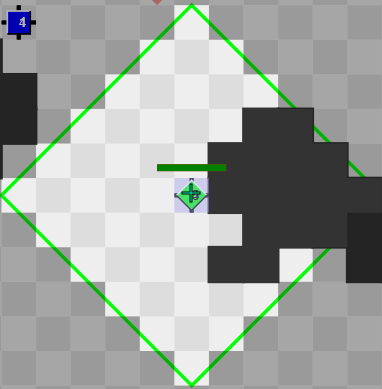
\includegraphics[width=120px]{bilder/agentensicht}
		\caption{Sicht des \textit{Agents}}
		\label{fig:agentensicht}
	\end{minipage}
\end{figure}

Im ersten Schritt ermittelt der \textit{Agent} einen möglichen Weg, wie er zu seinem Ziel gelangt. Hierfür wird der entsprechende Wegalgorithmus verwendet, welcher in Kapitel \textit{\ref{kap:wegfindung}} genauer erläutert wird. Sobald der Weg ermittelt wurde und bevor ein Schritt des Weges beschritten wird, prüft der \textit{Agent} auf Aktionen, welche vorher ausgeführt werden müssen. Diese Aktionen können einen Rollenwechseln beinhalten, ungenutzte Blöcke fallen lassen, einen Block vom \textit{Dispenser} anfordern oder einen Block aufnehmen, eine Aufgabe in der Endzone abgeben oder sich mit einem anderen \textit{Agents} verbinden. Diese Aktionen sind Momentaufnahmen, die der \textit{Agent} ausführen muss, bevor er zu einem neuen Ziel geht. Wenn keine dieser Aktionen passt, wird der \textit{Agent} den Weg zu seinem Ziel gehen. Hier kommt nochmals eine Entscheidungsmöglichkeit für den \textit{Agents} in Frage. Ist der nächste Schritt frei und ich kann den Weg gehen, dann geht er diesen. Sollte aber beispielsweise ein Block in der Richtung sein, in die der \textit{Agent} gehen möchte, so muss er diesen zunächst zerstören. Wenn ein \textit{Agent} in der Richtung steht, so wird ein Weg um diesen \textit{Agents} herum erstellt. In Abbildung \ref{fig:agentensicht} wäre der Weg in Richtung Westen durch einen Block gehindert, sodass er diesen zunächst zerstören muss, bevor er in diese Richtung gehen kann. 

Zusammengefasst muss der \textit{Agent} in jedem Schritt entscheiden, ob es eine Aktion gibt, die gerade notwendig ist, wie einen Block aufzunehmen oder ob der Schritt, den er gehen möchte, möglich ist.  

\subsection{Synchronisation und Kommunikation} \label{kap:kommunikation}
Die Kommunikation der \textit{Agents} funktioniert, sobald sie sich in einer Gruppe befinden. Die Synchronisation der Gruppen ist in Kapitel \textit{\ref{kap:Gruppenbildung}} genauer beschrieben. Für die Kommunikation wurde eine Schnittstelle entwickelt, welche die Nachricht, den Senderagenten und den Empfängeragenten in einer Nachrichtenbox bereithält. Stehen zwei \textit{Agents} um einen \textit{Dispenser} und beide möchten einen Block anfordern, so wird der Agent zunächst prüfen, ob eine Nachricht für ihn vorliegt. Ist dies nicht der Fall untersucht der Agent, ob andere, zu dem Team gehörende \textit{Agents,} in der nähe des \textit{Dispenser} stehen. Wenn die Prüfung erfolgreich ist, so wird er eine Nachricht an den \textit{Agent} senden und dieser wird dann warten, bis der \textit{Dispenser} frei ist. Er selbst stellt eine Anfrage an den \textit{Dispenser} und nimmt den Block dann auf.
